\chapter{Robotics: From Sensor Readings to Actions}
\label{ch:robotics}

\chapterguide%
  {Know what a classifier is, what a train/test split is for, and how to read a confusion matrix.}
  {describe the sense--think--act loop; explain wall following as a reactive policy; turn logged sensor data into a supervised control problem; read a decision tree as a set of threshold rules; evaluate a controller with the right metrics; and state why offline accuracy is not the same as safe control.}

The maze robot of Chapter~\ref{ch:uninformed} had a perfect map and all the time it wanted to plan. A real robot often has neither. Lab~5 studies the decision stage of one: a SCITOS G5 robot logged 5,456 readings from 24 ultrasonic sensors alongside the actions of a wall-following controller. The lab learns readable if--then rules from that log and compares them with a more powerful, opaque model.

\section{The sense--think--act loop}

Every robot runs some version of the same cycle. Sensors measure the world, a controller selects a command, and actuators change what the sensors will see next (\figref{fig:sta-loop}). The ``think'' box can be simple rules, a lookup table, a classifier, or a planner such as A$^\star$ (\chapref{ch:informed}).

\begin{utpfig}[The sense--think--act loop]{Lab~5 learns the ``think'' stage from sensor--action pairs. The dashed feedback arrow, actions changing future readings, is not tested offline.}{fig:sta-loop}
\begin{tikzpicture}[font=\small]
\node[utpbox,minimum width=2.9cm,minimum height=1.1cm] (sense) at (0,0) {\textbf{Sense}\\24 ultrasonic distances};
\node[utpbox,minimum width=2.9cm,minimum height=1.1cm,fill=UTPPaleOrange,draw=UTPOrange,line width=1pt] (think) at (4.6,0) {\textbf{Think}\\readings $\to$ action};
\node[utpbox,minimum width=2.9cm,minimum height=1.1cm] (act) at (9.2,0) {\textbf{Act}\\one of four motions};
\node[utpbox,minimum width=3.4cm,minimum height=0.9cm,fill=UTPPaleGray,draw=UTPMuted] (world) at (4.6,-2.2) {the room: walls, corners, doorways};
\draw[utparrow] (sense)--(think);
\draw[utparrow] (think)--(act);
\draw[utparrow] (act.south) |- (world.east);
\draw[utparrow,dashed] (world.west) -| (sense.south);
\node[utplabel,anchor=south,color=UTPOrange] at (4.6,0.75) {Lab~5: this box is learned from 5,456 logged pairs};
\node[utplabel,anchor=north,color=UTPMuted] at (4.6,-2.72) {dashed arrow: feedback, the next reading depends on this action};
\end{tikzpicture}
\end{utpfig}

\begin{intuition}
Offline control looks like classification: 24 readings in, one of four actions out. On a real robot, however, a wrong action can lead to situations the training data never contained.
\end{intuition}

\section{Wall following as a reactive policy}

\term{Wall following} keeps a robot moving along a wall at a fixed distance. In this dataset the robot circled the room clockwise, so the wall stayed on its left. Sensors on the wall side read short distances, and the others read open space, corners and doorways (\figref{fig:sensor-ring}).

\begin{analogy}
Walk down a dark corridor with one hand on the wall. You need no map and no memory of how far you have come. If your hand presses hard, you edge away; if it loses contact, you edge back. That is a \term{reactive} controller: every decision comes from the current reading alone.
\end{analogy}

\begin{utpfig}[The ultrasonic ring and the wall-following task]{The SCITOS robot from above, moving to the right with the wall on its left. Its 24 sensors are numbered clockwise from US00 at the front. The four that Lab~5 selects (orange) sit on the rear-left arc, where they measure the wall from slightly different angles.}{fig:sensor-ring}
\begin{tikzpicture}[font=\small]
\draw[line width=2.2pt,draw=UTPMuted] (-4.6,3.15) -- (4.6,3.15);
\node[utplabel,anchor=south,color=UTPMuted] at (-3.9,3.2) {wall, on the robot's left};
\draw[fill=UTPPaleBlue,draw=UTPBlue,line width=1pt] (0,0) circle (1.25);
\node[font=\scriptsize\bfseries\color{UTPNavy}] at (0,0.15) {SCITOS};
\node[font=\scriptsize\color{UTPMuted}] at (0,-0.2) {24 sensors};
\foreach \i in {0,...,23}{
  \pgfmathsetmacro{\ang}{-\i*15}
  \draw[draw=UTPBlue,thick] ({1.25*cos(\ang)},{1.25*sin(\ang)}) -- ({1.5*cos(\ang)},{1.5*sin(\ang)});
}
\foreach \i/\lbl in {13/US13,14/US14,17/US17,18/US18}{
  \pgfmathsetmacro{\ang}{-\i*15}
  \draw[draw=UTPOrange,line width=1.8pt] ({1.25*cos(\ang)},{1.25*sin(\ang)}) -- ({1.62*cos(\ang)},{1.62*sin(\ang)});
  \node[font=\tiny\bfseries\color{UTPOrange!85!black}] at ({1.98*cos(\ang)},{1.92*sin(\ang)}) {\lbl};
}
\draw[utpptr,draw=UTPOrange] (0,2.1) -- (0,3.08);
\draw[utpptr,draw=UTPOrange] (-0.56,2.05) -- (-0.82,3.08);
\node[utplabel,anchor=west,color=UTPOrange!85!black,align=left] at (0.2,2.6) {short readings on the wall side};
\node[font=\tiny\bfseries\color{UTPNavy},anchor=west] at (1.55,0) {US00};
\draw[utparrow,draw=UTPGreen,line width=1.2pt] (2.15,0) -- (3.45,0);
\node[utplabel,anchor=north west,align=left,color=UTPGreen!80!black] at (1.65,-0.12) {heading; turning right\\moves away from the wall};
\node[utplabel,anchor=north,align=center,color=UTPMuted] at (0,-1.6) {the four actions: Move-Forward, Slight-Left-Turn,\\Slight-Right-Turn, Sharp-Right-Turn};
\end{tikzpicture}
\end{utpfig}

Written as rules, the natural controller for this task is short:

\begin{itemize}
  \item If the wall-side distance is very short, turn sharply away from the wall.
  \item If it is a little short, turn slightly away; if a little long, turn slightly towards.
  \item Otherwise, move forward.
\end{itemize}

These rules are cheap and auditable, but they need thresholds. What counts as ``very short''? Lab~5 learns the answer from data.

\section{Learning a controller from logged behaviour}

Ask one question of any dataset: \emph{does your log hold the answers?} Here it does. Each row records what the sensors read and what the controller did, so this is \term{supervised} learning. Ask a second question: \emph{is the answer a number or a category?} Here it is one of four actions, so the job is \term{classification} rather than regression. Learning a policy from such demonstrations has a name, \term{behavioural cloning}: supervised classification with 24 features and four classes.

\begin{analogy}
Think of learning to drive by watching an instructor. You see thousands of moments of good driving and copy them. That works until you drift a little off-centre, because the instructor never drifted, so you have never seen what to do from there.
\end{analogy}

Three properties of the data shape what we do next.

\begin{description}
  \item[The classes are imbalanced.] Move-Forward accounts for 40\,\% of rows, Sharp-Right-Turn 38\,\%, Slight-Right-Turn 15\,\% and Slight-Left-Turn 6\,\%. A controller that never turned slightly left could still reach 94\,\% accuracy. So report \term{macro F1}, which weights classes equally, and train with \texttt{class\_weight="balanced"}.
  \item[Consecutive rows are not independent.] Neighbouring readings resemble each other, which makes the lab's random-split test score optimistic. The noise experiment probes robustness beyond this split.
  \item[Test rows are held back.] Save a seeded, stratified 70/30 split first. Select features, tune depth and fit the reference model on training rows, and evaluate on test rows only in Question~5.
\end{description}

\subsection{Choosing the sensors}

Not all 24 sensors matter equally. Rank them by \term{mutual information} with the action, using training rows only, and keep the top four: US14, US17, US18 and US13, a cluster on the wall side. Mutual information measures how much knowing a reading reduces your uncertainty about the action. A sensor pointing into open space tells you little; a sensor watching the wall tells you a lot.

\section{An interpretable controller: the decision tree}

A \term{decision tree} applies feature thresholds one at a time until it reaches a class, like a game of twenty questions. Each path from the root to a leaf reads as one if--then rule learned from the demonstrations (\figref{fig:tree-rules}).

\begin{utpfig}[A decision tree is a list of threshold rules]{The learned tree\textquotesingle s top three levels and three example rules. Nodes test sensor thresholds; leaves select actions. Limiting depth keeps the rules readable.}{fig:tree-rules}
\begin{tikzpicture}[font=\small,
  q/.style={draw=UTPBlue,fill=UTPPaleBlue,rounded corners=1.5mm,minimum width=2.3cm,minimum height=0.7cm,align=center,font=\scriptsize\color{UTPNavy}},
  a/.style={draw=UTPGreen,fill=UTPPaleTeal,rounded corners=1.5mm,minimum width=2.2cm,minimum height=0.6cm,align=center,font=\scriptsize\bfseries\color{UTPNavy}},
  m/.style={draw=UTPMuted!60,fill=UTPPaleGray,rounded corners=1.5mm,minimum width=2.2cm,minimum height=0.6cm,align=center,font=\scriptsize\color{UTPMuted}}]
\node[q] (r) at (0,0) {US14 $\le$ 0.90?};
\node[a] (l1) at (-2.4,-1.3) {Sharp-Right-Turn};
\node[q] (n1) at (2.4,-1.3) {US18 $\le$ 1.00?};
\node[q] (n2) at (0.6,-2.6) {US18 $\le$ 0.50?};
\node[q] (n3) at (4.2,-2.6) {US17 $\le$ 0.90?};
\node[m] (l2) at (0.3,-3.95) {$\cdots$ turns or\\forward};
\node[m] (l3) at (2.95,-3.95) {$\cdots$ forward or\\slight right};
\node[m] (l4) at (5.55,-3.95) {$\cdots$ mostly\\Slight-Left-Turn};
\draw[utpptr] (r)--(l1) node[midway,left,utplabel] {yes};
\draw[utpptr] (r)--(n1) node[midway,right,utplabel] {no};
\draw[utpptr] (n1)--(n2) node[midway,left,utplabel] {yes};
\draw[utpptr] (n1)--(n3) node[midway,right,utplabel] {no};
\draw[utpptr] (n2)--(l2);
\draw[utpptr] (n3)--(l3) node[midway,left,utplabel] {yes};
\draw[utpptr] (n3)--(l4) node[midway,right,utplabel] {no};
\node[utplabel,anchor=west,align=left,text width=5.2cm] at (7.0,-2.0)
  {\textbf{Three paths as rules}\\[3pt]
   IF US14 $\le$ 0.90\,m THEN Sharp-Right-Turn\\[2pt]
   IF US14 $>$ 0.90 AND US18 $>$ 1.00 AND US17 $\le$ 0.79 THEN Move-Forward\\[2pt]
   IF US14 $>$ 0.90 AND US18 $>$ 1.00 AND $0.79<$ US17 $\le 0.90$ THEN Slight-Right-Turn\\[3pt]
   14 leaves in total at depth~5; the full list is \texttt{rule\_controller.txt}.};
\end{tikzpicture}
\end{utpfig}

The first split is the wall-following reflex itself: \emph{if the wall-side sensor reads less than 0.9\,m, turn sharply right, away from the wall}. Nobody typed that threshold. It was found in the demonstrations.

\subsection{Choosing the depth}

A deeper tree fits the training rows better and reads worse. The lab treats depth as a hyperparameter and picks it without touching the test rows: it carves a validation set out of the training rows, trains trees of depth 2 to 6 on the remainder, and scores each on the validation set. Macro F1 climbs steeply from depth~2 ($0.46$) to depth~4 ($0.87$), reaches $0.89$ at depth~5 and stops improving. Depth~5 is selected, the tree is refitted on all training rows, and \texttt{export\_text} writes it out as the rule list saved in \texttt{rule\_controller.txt}.

\begin{keyidea}
Interpretability is a design constraint, not a by-product. The lab fixes the number of sensors and caps the tree depth \emph{before} training, then measures what those constraints cost. Loosening either would raise the score and lose the ability to read the controller.
\end{keyidea}

\section{A reference model and a fair comparison}

The reference \term{random forest} uses 200 trees, each trained on a bootstrap sample of the rows, with all 24 sensors. Instead of one readable note, you consult two hundred advisers and take a vote. It shows what the compact rule tree gives up. Evaluate both on the same held-out rows.

\begin{utptable}
\begin{tabularx}{\linewidth}{@{}>{\bfseries\leavevmode\color{UTPNavy}}m{0.30\linewidth}>{\centering\arraybackslash}X>{\centering\arraybackslash}X>{\centering\arraybackslash}X>{\centering\arraybackslash}X@{}}
\toprule
\rowcolor{UTPPaleBlue!92}
\utpth{Model} & \utpth{Accuracy} & \utpth{Macro precision} & \utpth{Macro recall} & \utpth{Macro F1} \\
\midrule
Rule tree, 4 sensors, depth 5 & 0.923 & 0.879 & 0.921 & 0.895 \\
Random forest, 24 sensors & 0.995 & 0.993 & 0.992 & 0.992 \\
\bottomrule
\end{tabularx}
\end{utptable}

The readable controller sacrifices seven percentage points of accuracy and ten of macro F1. Whether that is acceptable depends on how much you need to audit its behaviour.

\subsection{Reading the confusion matrix}

A headline score does not tell you which mistakes a controller makes, and on a robot some mistakes are worse than others. \figref{fig:confusion-rule} gives the rule tree's test results. Read along a row to see what happened to one true action, and down a column to see what one predicted action really was.

\begin{utpfig}[The rule tree's confusion matrix]{The rule tree on 1,637 test rows. Rows are the true action and columns the prediction, so the diagonal counts correct decisions. Recall reads along a row and precision down a column.}{fig:confusion-rule}
\begin{tikzpicture}[font=\small,
  hit/.style={draw=UTPGreen,fill=UTPGreen!28,minimum width=1.55cm,minimum height=0.72cm,font=\small\bfseries\color{UTPNavy}},
  miss/.style={draw=UTPMuted!30,fill=white,minimum width=1.55cm,minimum height=0.72cm,font=\small\color{UTPMuted}},
  bad/.style={draw=UTPRed,fill=UTPPaleRed,minimum width=1.55cm,minimum height=0.72cm,font=\small\bfseries\color{UTPRed}},
  rowlab/.style={anchor=east,font=\scriptsize\color{UTPNavy}},
  collab/.style={anchor=south,font=\scriptsize\color{UTPNavy},align=center}]
\def\cw{1.6}\def\ch{0.76}
\foreach \name [count=\i from 0] in {Move-\\Forward,Sharp\\Right,Slight\\Right,Slight\\Left}{\node[collab] at (\cw*\i,0.42) {\name};}
\foreach \name [count=\i from 0] in {true Move-Forward,true Sharp-Right,true Slight-Right,true Slight-Left}{\node[rowlab] at (-0.9,-\ch*\i) {\name};}
\node[hit] at (0,0) {624};\node[miss] at (\cw,0) {0};\node[miss] at (2*\cw,0) {12};\node[miss] at (3*\cw,0) {26};
\node[bad] at (0,-\ch) {36};\node[hit] at (\cw,-\ch) {574};\node[miss] at (2*\cw,-\ch) {11};\node[miss] at (3*\cw,-\ch) {8};
\node[miss] at (0,-2*\ch) {22};\node[miss] at (\cw,-2*\ch) {0};\node[hit] at (2*\cw,-2*\ch) {221};\node[miss] at (3*\cw,-2*\ch) {5};
\node[miss] at (0,-3*\ch) {6};\node[miss] at (\cw,-3*\ch) {0};\node[miss] at (2*\cw,-3*\ch) {0};\node[hit] at (3*\cw,-3*\ch) {92};
\foreach \r/\y in {0.94/0,0.91/-1,0.89/-2,0.94/-3}{\node[font=\scriptsize\color{UTPNavy},anchor=west] at (3*\cw+0.9,\ch*\y) {\r};}
\node[font=\scriptsize\bfseries\color{UTPNavy},anchor=south] at (3*\cw+1.2,0.42) {recall};
\foreach \p/\x in {0.91/0,1.00/1,0.91/2,0.70/3}{\node[font=\scriptsize\color{UTPNavy},anchor=north] at (\cw*\x,-3*\ch-0.4) {\p};}
\node[font=\scriptsize\bfseries\color{UTPNavy},anchor=east] at (-0.9,-3*\ch-0.57) {precision};
\end{tikzpicture}
\end{utpfig}

Three things stand out. Slight-Right-Turn has the lowest recall, $0.89$, and 22 of its 27 misses were called Move-Forward: the line between ``keep going'' and ``nudge right'' sits on thresholds such as US17 at 0.79\,m and 0.90\,m, and a reading a few centimetres away flips the action. Slight-Left-Turn has the lowest precision, $0.70$, because balanced class weights push the tree towards this rare action, so 39 of its 131 predictions were wrong. And the red cell deserves the most attention. In 36 test rows the robot should have turned sharply away from the wall and was told to carry on forward. Accuracy counts that the same as any other miss, but an engineer would not.

\section{Robustness: what noise does to thresholds}

Ultrasonic readings are noisy, and noise can move a reading across a threshold: 0.90\,m may become 0.87 or 0.93\,m. Lab~5 adds Gaussian noise at 2, 5 and 10\,\% of each selected sensor's training standard deviation to the test readings. Test macro F1 falls quickly.

\begin{utptable}
\begin{tabularx}{\linewidth}{@{}>{\bfseries\leavevmode\color{UTPNavy}}m{0.34\linewidth}>{\centering\arraybackslash}X>{\centering\arraybackslash}X>{\centering\arraybackslash}X>{\centering\arraybackslash}X@{}}
\toprule
\rowcolor{UTPPaleBlue!92}
\utpth{Noise, as a fraction of training SD} & \utpth{0} & \utpth{2\,\%} & \utpth{5\,\%} & \utpth{10\,\%} \\
\midrule
Rule-tree macro F1 & 0.895 & 0.858 & 0.787 & 0.706 \\
\bottomrule
\end{tabularx}
\end{utptable}

Possible responses all trade simplicity for robustness: more sensors provide redundancy, deeper trees allow finer partitions, and ensembles combine many decisions. For a 5\,\% noise budget, you should be able to justify one choice and state its cost.

\begin{pitfall}
Noise added only to \emph{test} readings measures the robustness of a controller trained on clean data. Training on noisy data is a different experiment. State which one you ran.
\end{pitfall}

\section{From offline accuracy to safe control}

Four factors separate evaluation on a fixed table from a running robot:

\begin{description}
  \item[Feedback.] A wrong action changes the readings that follow and may lead outside the training distribution, where errors compound (\figref{fig:drift}).
  \item[Timing.] Sensor, computation and motor delays can make a correct decision act on an outdated reading.
  \item[Failure modes.] Sensor failures or sound-absorbing walls can produce unfamiliar readings that the classifier still labels confidently.
  \item[Safety limits.] Minimum distances, speed caps and emergency stops must constrain the learned policy. Accuracy does not measure them.
\end{description}

\begin{utpfig}[Small errors compound under feedback]{The shaded band is what the demonstrations covered. The learned controller makes a small mistake, drifts to the edge of that band, and then meets readings it was never trained on, so its next mistakes grow. A table of logged rows cannot show this, because the table never changes in response to a prediction.}{fig:drift}
\begin{tikzpicture}[font=\small]
\fill[UTPTeal!16] (0,-0.5) rectangle (10.5,0.5);
\node[utplabel,anchor=west,color=UTPTeal!70!black] at (0.1,0.72) {states seen in the demonstrations};
\draw[line width=2.2pt,draw=UTPMuted] (0,1.35) -- (10.5,1.35);
\node[utplabel,anchor=west,color=UTPMuted] at (8.9,1.52) {wall};
\draw[draw=UTPGreen,line width=1.3pt,-{Stealth[length=2mm]}] (0,0) -- (10.4,0);
\node[utplabel,anchor=north east,color=UTPGreen!80!black] at (10.4,-0.05) {the demonstrated path};
\draw[draw=UTPRed,line width=1.3pt,-{Stealth[length=2mm]}] plot[smooth,tension=0.6] coordinates {(0,0) (2,0.02) (3.5,0.14) (5,0.42) (6.2,0.72) (7.2,1.02) (7.9,1.28)};
\node[utplabel,anchor=north,color=UTPRed,align=center] at (5.6,-0.6) {learned controller: one small error, then unfamiliar readings};
\node[circle,fill=UTPRed,inner sep=1.3pt] at (3.5,0.14) {};
\node[utplabel,anchor=south,color=UTPRed] at (3.25,0.2) {first error};
\end{tikzpicture}
\end{utpfig}

The rule tree is an offline \emph{perception-to-action prototype}, not a validated robot controller. Its readability is what supports the closed-loop testing it would need next.

\begin{chapterrecap}
\begin{itemize}
  \item Robots repeat sense, think, act, and actions change what is sensed next.
  \item Wall following is a reactive policy, and behavioural cloning learns one from logged demonstrations as a classification problem.
  \item A shallow decision tree is a readable list of threshold rules; a random forest shows what readability costs.
  \item Macro F1 and the confusion matrix say which actions fail, and that matters more than overall accuracy when errors differ in danger.
  \item Offline accuracy cannot see feedback, delays, sensor failure or safety limits.
\end{itemize}
\end{chapterrecap}

\begin{quickcheck}
\begin{enumerate}
  \item Why does Lab~5 report macro F1 rather than accuracy, and what accuracy could a controller that never predicts Slight-Left-Turn achieve?
  \item Feature selection and depth tuning both use only the training rows. What would be wrong with the test score if the four sensors had been chosen on all rows?
  \item Write the first rule of the learned tree in plain English and say what physical situation it responds to.
  \item Which action has the lowest recall for the rule tree, and what does \figref{fig:confusion-rule} say about where its misses go?
  \item Name one reason a controller with 92\,\% offline accuracy could still drive a robot into a wall.
\end{enumerate}
\end{quickcheck}


\labsection{5}{Robotics: Sensor-to-Action Control}{sec:lab05-robotics}

\begin{labproject}{Build and evaluate an interpretable wall-following controller}
\textbf{Read first.} Chapter~\ref{ch:robotics}.\\
\textbf{Goal.} Derive a four-sensor threshold policy, compare it with an all-sensor reference model, and test its sensitivity to sensor noise.\\
\textbf{Scenario.} A SCITOS G5 robot must convert 24 ultrasonic readings into one of four movement commands while following a wall.\\
\textbf{Data.} \texttt{all\_datasets/lab05-sensor\_readings\_24.csv} (5,456 readings, no header: 24 distances in metres, then the action).\\
\textbf{Notebook.} \texttt{all\_experiments/lab05\_robotics\_sensor\_control\_worked.ipynb}.\\
\textbf{Hand in.} The executed notebook, the \texttt{results/lab05/} folder and a short conclusion, as listed in the checklist at the end of this sheet.
\end{labproject}

\begin{labmode}
\begin{enumerate}
  \item Activate your course environment and confirm that the data file is in \texttt{all\_datasets/}.
  \item Start Jupyter from \texttt{all\_experiments/}, open the notebook, and choose \textbf{Restart Kernel and Run All Cells}. Everything runs in a few seconds.
\end{enumerate}
\begin{lstlisting}[style=utpterminal]
cd all_experiments
jupyter lab
\end{lstlisting}
Prefer a plain script? From the course folder, \texttt{python all\_experiments/lab05\_robotics\_sensor\_control\_worked.py} runs the same code and writes the same evidence.
\end{labmode}

\courselabflow{Split readings}{Select sensors}{Fit controller}{Test noise}


\labroutine

\begin{yourturn}
\textbf{Warm-up on paper.} Using the first levels of the learned tree in \figref{fig:tree-rules}, decide what the controller does for these readings: (a) US14 $=0.81$; (b) US14 $=1.94$, US18 $=5.00$, US17 $=1.44$. Say in plain words what is happening around the robot in each case.

\emph{Answer.} (a) Sharp-Right-Turn: the wall is close on the rear left, so steer away. (b) US14 and US18 are both large and US17 is above 0.90, so the tree goes down the branch that mostly says Slight-Left-Turn: the wall has fallen away, so edge back towards it.
\end{yourturn}

\textbf{Setup.} Run the imports and path setup first, and keep this kernel state for the later questions. In the script version the first seven lines also set the working directory.
\lstinputlisting[style=utppython,firstline=1,lastline=7]{all_experiments/lab05_robotics_sensor_control_worked.py}
\lstinputlisting[style=utppython,firstline=8,lastline=23]{all_experiments/lab05_robotics_sensor_control_worked.py}

\begin{labquestion}{1}{Inspect the data and fix the split}
The CSV has no header: 24 ultrasonic distances (metres) followed by the action label. Name the columns, report the class balance and sensor summary statistics, and create a fixed stratified 70/30 train/test split with seed 42. Save the split.
\end{labquestion}
\begin{labanswer}
\courselabtrace{Protect the evaluation boundary}{Training}{Select four sensors and learn thresholds}{Test}{Apply the frozen policy to unseen readings}{Noise}{Perturb test sensors; keep labels unchanged}

\lstinputlisting[style=utppython,firstline=25,lastline=38]{all_experiments/lab05_robotics_sensor_control_worked.py}
\begin{refoutput}
\begin{lstlisting}[style=utpterminal]
Shape: (5456, 25)
Move-Forward 2205 (0.404)   Sharp-Right-Turn 2097 (0.384)
Slight-Right-Turn 826 (0.151)   Slight-Left-Turn 328 (0.060)
{'train': 3819, 'test': 1637}
\end{lstlisting}
\end{refoutput}

\textbf{What it means.} The classes are imbalanced, so accuracy alone would flatter a model that ignores the small classes, and macro F1 is reported throughout. Sensor readings are distances in metres between 0.4~m and 5~m. Stratification keeps the class shares equal in the 3,819 training and 1,637 test rows. The notebook numbers the sensors from US00, the front sensor, clockwise to US23.
\end{labanswer}

\begin{labquestion}{2}{Select four sensors using training data only}
Rank the 24 sensors by mutual information with the action, computed on the training rows only, and keep the top four for the interpretable controller. Save the full ranking.
\end{labquestion}
\begin{labanswer}
Read \texttt{selected} rather than hard-coding the names from a saved run:
\courselabtrace{Trace training-only sensor selection}{1. Input / state}{X has US00 through US23; train\_idx and test\_idx preserve the stratified split.}{2. Operation}{Compute mi on X.loc[train\_idx] and training actions; sort feature\_table and take its first four sensor names.}{3. Check}{selected is reused, in the same order, for tree fitting and held-out predictions.}


\lstinputlisting[style=utppython,firstline=40,lastline=45]{all_experiments/lab05_robotics_sensor_control_worked.py}
\begin{refoutput}
\begin{lstlisting}[style=utpterminal]
Selected sensors: ['US14', 'US17', 'US18', 'US13']
\end{lstlisting}
\end{refoutput}

\textbf{What it means.} The four most informative sensors come from the same rear-left arc of the ring, which is what a wall follower needs: the distance to the wall it is tracking, seen from slightly different angles. Selecting on training rows only keeps the test set untouched.
\end{labanswer}

\textbf{Connect it to the chapter.} The next questions fill in the ``think'' box of this loop. Remember that the dashed arrow is not tested here.
% Reused from chapters/05-robotics-scenarios.tex
\begin{labvisual}{Recall the chapter model}
\begin{labgraphic}
\begin{tikzpicture}[font=\small]
\node[utpbox,minimum width=2.9cm,minimum height=1.1cm] (sense) at (0,0) {\textbf{Sense}\\24 ultrasonic distances};
\node[utpbox,minimum width=2.9cm,minimum height=1.1cm,fill=UTPPaleOrange,draw=UTPOrange,line width=1pt] (think) at (4.6,0) {\textbf{Think}\\readings $\to$ action};
\node[utpbox,minimum width=2.9cm,minimum height=1.1cm] (act) at (9.2,0) {\textbf{Act}\\one of four motions};
\node[utpbox,minimum width=3.4cm,minimum height=0.9cm,fill=UTPPaleGray,draw=UTPMuted] (world) at (4.6,-2.2) {the room: walls, corners, doorways};
\draw[utparrow] (sense)--(think);
\draw[utparrow] (think)--(act);
\draw[utparrow] (act.south) |- (world.east);
\draw[utparrow,dashed] (world.west) -| (sense.south);
\node[utplabel,anchor=south,color=UTPOrange] at (4.6,0.75) {Lab~5: this box is learned from 5,456 logged pairs};
\node[utplabel,anchor=north,color=UTPMuted] at (4.6,-2.72) {dashed arrow: feedback --- the next reading depends on this action};
\end{tikzpicture}
\end{labgraphic}\end{labvisual}


\begin{labquestion}{3}{Fit an interpretable rule controller}
A shallow decision tree is a fixed set of threshold rules. Carve an internal validation set out of the training rows, choose the tree depth by validation macro F1, refit on all training rows, and export the final tree as explicit if--then rules.
\end{labquestion}
\begin{labanswer}
\lstinputlisting[style=utppython,firstline=47,lastline=65]{all_experiments/lab05_robotics_sensor_control_worked.py}
\begin{refoutput}
\begin{lstlisting}[style=utpterminal]
depth 2: 0.463   depth 3: 0.826   depth 4: 0.872   depth 5: 0.887   depth 6: 0.883
Selected depth: 5 | leaves: 14
|--- US14 <= 0.90
|   |--- class: Sharp-Right-Turn
|--- US14 >  0.90
|   |--- US18 <= 1.00
...
\end{lstlisting}
\end{refoutput}

\textbf{What it means.} Validation macro F1 climbs steeply from depth 2 to 4 and flattens at depth 5, which is selected. The exported tree reads as a policy. Its very first split, \emph{if the wall-side sensor US14 reads less than 0.9~m, turn sharply right}, is the wall-following reflex, and the deeper splits refine the slight turns. Every decision is a threshold a robotics engineer can inspect.
\end{labanswer}

\begin{labquestion}{4}{Fit a reference model}
Train a random forest on all 24 sensors using the same training partition. It is not interpretable; its purpose is to show what accuracy the four-sensor rule controller gives up.
\end{labquestion}
\begin{labanswer}
\lstinputlisting[style=utppython,firstline=67,lastline=70]{all_experiments/lab05_robotics_sensor_control_worked.py}
\begin{refoutput}
\begin{lstlisting}[style=utpterminal]
Random forest trained on 24 sensors with 200 trees
\end{lstlisting}
\end{refoutput}

\textbf{What it means.} The forest uses every sensor and 200 trees, so it can exploit interactions the shallow tree cannot. It is the reference ceiling, not a candidate controller.
\end{labanswer}

\begin{labquestion}{5}{Evaluate on the held-out data}
Report accuracy, macro precision, macro recall and macro F1 for both models on the test rows, draw both confusion matrices, list per-class recall for the rule controller, and identify its hardest action.
\end{labquestion}
\begin{labanswer}
\lstinputlisting[style=utppython,firstline=72,lastline=97]{all_experiments/lab05_robotics_sensor_control_worked.py}
\begin{labvisual}{Reference plot from the supplied notebook}
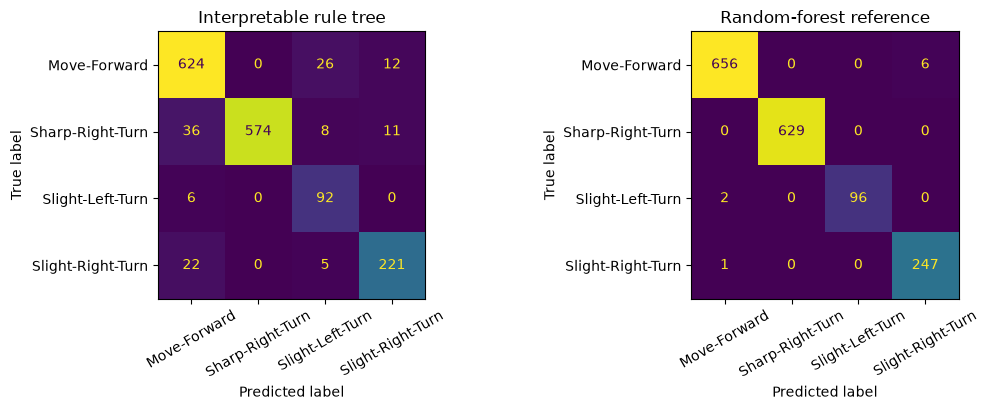
\includegraphics[width=.88\linewidth,height=5cm,keepaspectratio]{labs/visuals/05-notebook-reference.png}
\end{labvisual}
\begin{refoutput}
\begin{lstlisting}[style=utpterminal]
                     model  accuracy  macro_precision  macro_recall  macro_f1
0  Interpretable rule tree     0.923            0.879         0.921     0.895
1  Random-forest reference     0.995            0.993         0.992     0.992
Hardest action for the rule controller (lowest recall): Slight-Right-Turn
\end{lstlisting}
\end{refoutput}

\textbf{What it means.} The four-sensor tree reaches about 92\,\% accuracy and 0.90 macro F1; the all-sensor forest reaches over 99\,\% on both. The rule controller's weakest action is Slight-Right-Turn, and 22 of its 27 misses are called Move-Forward: the line between carrying on and nudging right sits on thresholds that a few centimetres can cross. That is the accuracy cost of a controller a person can read.
\end{labanswer}

\begin{labquestion}{6}{Test robustness to sensor noise}
Add zero-mean Gaussian noise to the test readings at 2, 5 and 10\,\% of the training-set standard deviation of each selected sensor, and plot the rule controller's macro F1 against the noise level.
\end{labquestion}
\begin{labanswer}
\lstinputlisting[style=utppython,firstline=99,lastline=116]{all_experiments/lab05_robotics_sensor_control_worked.py}
\begin{refoutput}
\begin{lstlisting}[style=utpterminal]
noise   0%: 0.895     2%: 0.858     5%: 0.787     10%: 0.706
Saved: ['confusion_matrices.png', 'feature_scores.csv', 'metrics.csv', 'noise_robustness.csv', 'noise_robustness.png', 'rule_controller.txt', 'rule_per_class.csv', 'split.csv']
\end{lstlisting}
\end{refoutput}

\textbf{What it means.} Macro F1 falls steadily as noise pushes readings across thresholds. Even 5\,\% of one standard deviation costs about eleven points, because a hard threshold has no margin: a reading on the wrong side by one millimetre gets the other action.
\end{labanswer}

\begin{yourturn}
Add new cells at the end of the notebook for these three tasks.
\begin{enumerate}
  \item \textbf{Trace one test row.} Row 265 reads US14 $=1.173$, US17 $=0.718$, US18 $=0.686$ and US13 $=5.0$. Follow it through \texttt{rule\_controller.txt} by hand, then confirm with \texttt{rule\_model.predict(X.loc[[265], selected])}. Now change US14 to $0.85$ in a copy of the row and predict the new action.
  \item \textbf{How many sensors?} Rerun the validation comparison at depth 5 with the top 1, 2, 4, 8 and 24 sensors from \texttt{feature\_table}. Use validation rows only. Where do extra sensors stop paying for themselves?
  \item \textbf{Respond to a 5\,\% noise budget.} Try two responses and compare their macro F1 on test readings with 5\,\% noise: retrain the four-sensor tree on noisy training readings, and fit a tree of depth 8 on the top eight sensors. State the cost of each.
\end{enumerate}
\end{yourturn}

\begin{expectedfindings}
\begin{enumerate}
  \item US14 $>0.90$; US18 $\le1.00$ and $>0.50$; US13 $>0.90$; US17 $>0.49$: \textbf{Move-Forward}, which is also the true action. With US14 at $0.85$ the very first rule fires: \textbf{Sharp-Right-Turn}.
  \item Validation macro F1 is 0.544, 0.803, 0.887, 0.943 and 0.967. The jump from one to four sensors is large, and after that each gain costs more sensors for less.
  \item Retraining the four-sensor tree on noisy readings barely helps (about 0.79 on noisy readings) and costs clean performance (about 0.83 on clean readings). Eight sensors at depth 8 give about 0.82 on noisy readings and 0.94 on clean readings, at the price of 23 leaves instead of 14 and twice the sensors to maintain. Your numbers will vary a little with the random seed for the noise.
\end{enumerate}
\end{expectedfindings}

\begin{troubleshoot}
\begin{description}
  \item[Sensor names look wrong] The file has no header, so \texttt{header=None} and \texttt{names=...} must both be present, as in Question~1.
  \item[A feature-name warning at \texttt{predict}] You passed a NumPy array to a model fitted on a DataFrame. Wrap it in \texttt{pd.DataFrame(values, columns=selected)}.
  \item[Test scores much higher than the reference] You probably selected sensors or depth using test rows. Check that every \texttt{fit} before Question~5 uses training rows only.
\end{description}
\end{troubleshoot}

\begin{verification}
\begin{itemize}
  \item The 5,456 readings are split 70/30 with stratification, and the split is saved.
  \item The four sensors are selected by mutual information on the training rows only.
  \item The tree depth is chosen by validation macro F1, and the final tree is exported as readable if--then rules.
  \item On the test rows the rule controller reaches about 92\,\% accuracy and 0.90 macro F1, and its hardest action is identified.
  \item Macro F1 is reported at every noise level, and you can explain why it falls.
\end{itemize}
\end{verification}

\begin{labdeliverable}
\begin{itemize}
  \item Restart the kernel and run all cells without errors.
  \item Submit the executed notebook, including your \emph{Your turn} cells, and the generated \texttt{results/lab05/} folder.
  \item Add a short conclusion: identify the hardest action, and recommend one response to a 5\,\% sensor-noise budget, including its trade-off.
\end{itemize}
\end{labdeliverable}

